\chapter{Install}
\label{chap:inst}

{\lpmd} had been probed in different architechtures and compilers. However in
the branch 0.6 and later the developers are only tested the code using two
principal architechtures :

\begin{itemize}
 \item Linux I686/AMD64 (Debian based architectures principally)
 \item OS/X
\end{itemize}

On the other hand {\lpmd} have the \index{lpmd-installer}\verb|lpmd-installer|
program, focused in the installation of {\lpmd} made simple over different
machines, wroted in python. We strongly recommend that beginners users use the
\verb|lpmd-installer| program to install {\lpmd} in the computer.

The basic requirements in order to install lpmd in a single computer are :

\begin{itemize}
 \item C++ compiler.(recomended 4.2 or later for GNU and 10.1 or later for
intel)
 \item zlib libraries. (recomended the more updated version)
 \item Python 2.7 or later. (suggested Python 3.0 for branch 0.7)
 \item If you want install lpvisual plugin and/or use lpmd-plotter, we suggest:
 \begin{itemize}
  \item OpenGL
  \item imagemagick
  \item mencoder
 \end{itemize}
\end{itemize} 

\section{lpmd-installer}

Is an program focused in a friendly installation of {\lpmd}, this program was
wroted in Python and is the manager in install in an automatic way the three
principal packages that are part of the lpmd program. These programs are :

\begin{itemize}
 \item liblpmd : Principal \index{API}API of the project.
 \item plugins : Plugins set for MD and Structure analysis.
 \item lpmd : Principal program with extra utilities.
\end{itemize}

\fb{
\begin{minipage}[l]{10cm}
If you don't like use the automatic installation process with
\texttt{lpmd-installer} go to the section~\ref{sec:descarga}.
\end{minipage}
}

\subsection{Instaling the lpmd-installer program}

Because \verb|lpmd-installer| is a python script, the installation of this
script is a very simple work, in order to have a correct functionability of
\verb|lpmd-installer| you will need :

\begin{itemize}
\item Python 2.7 or later.
\item Internet connection.
\end{itemize}

In order to install \verb|lpmd-installer| in the system you can use two
different ways. The first one is for distributions based in Debian (like
Ubuntu), for this case you can choose download the deb file only or add the
~\index{GNM}GNM ~\index{repository}repository to your system. The
second way is for different kind of distributions, in this case in necessary
download the program and install manually.

\subsubsection{Debian based distributions - download deb file}
You can directly download the deb file in internet and install using your
favorite tool. To download the deb file go to the web page :

\url{http://www.lpmd.cl/Download/lpmd-installer/}

\noindent
and download the las version available. To start the installation procedure, you
can open a terminal and install the package using dpkg command.

\begin{verbatim}
 user@machine:$ dpkg -i lpmd-installer.deb
\end{verbatim}

Or on the other hand you can make double-click on the package in a more
typical ubuntu system.

\begin{figure}[h!]
\centering
\subfigure[The deb package in the desktop.]
{
 
\includegraphics[scale=.20]{installer-package-1.pdf}
 \label{fig:installer-package-1}
}
\subfigure[Double click to the lpmd-installer package.]
{
 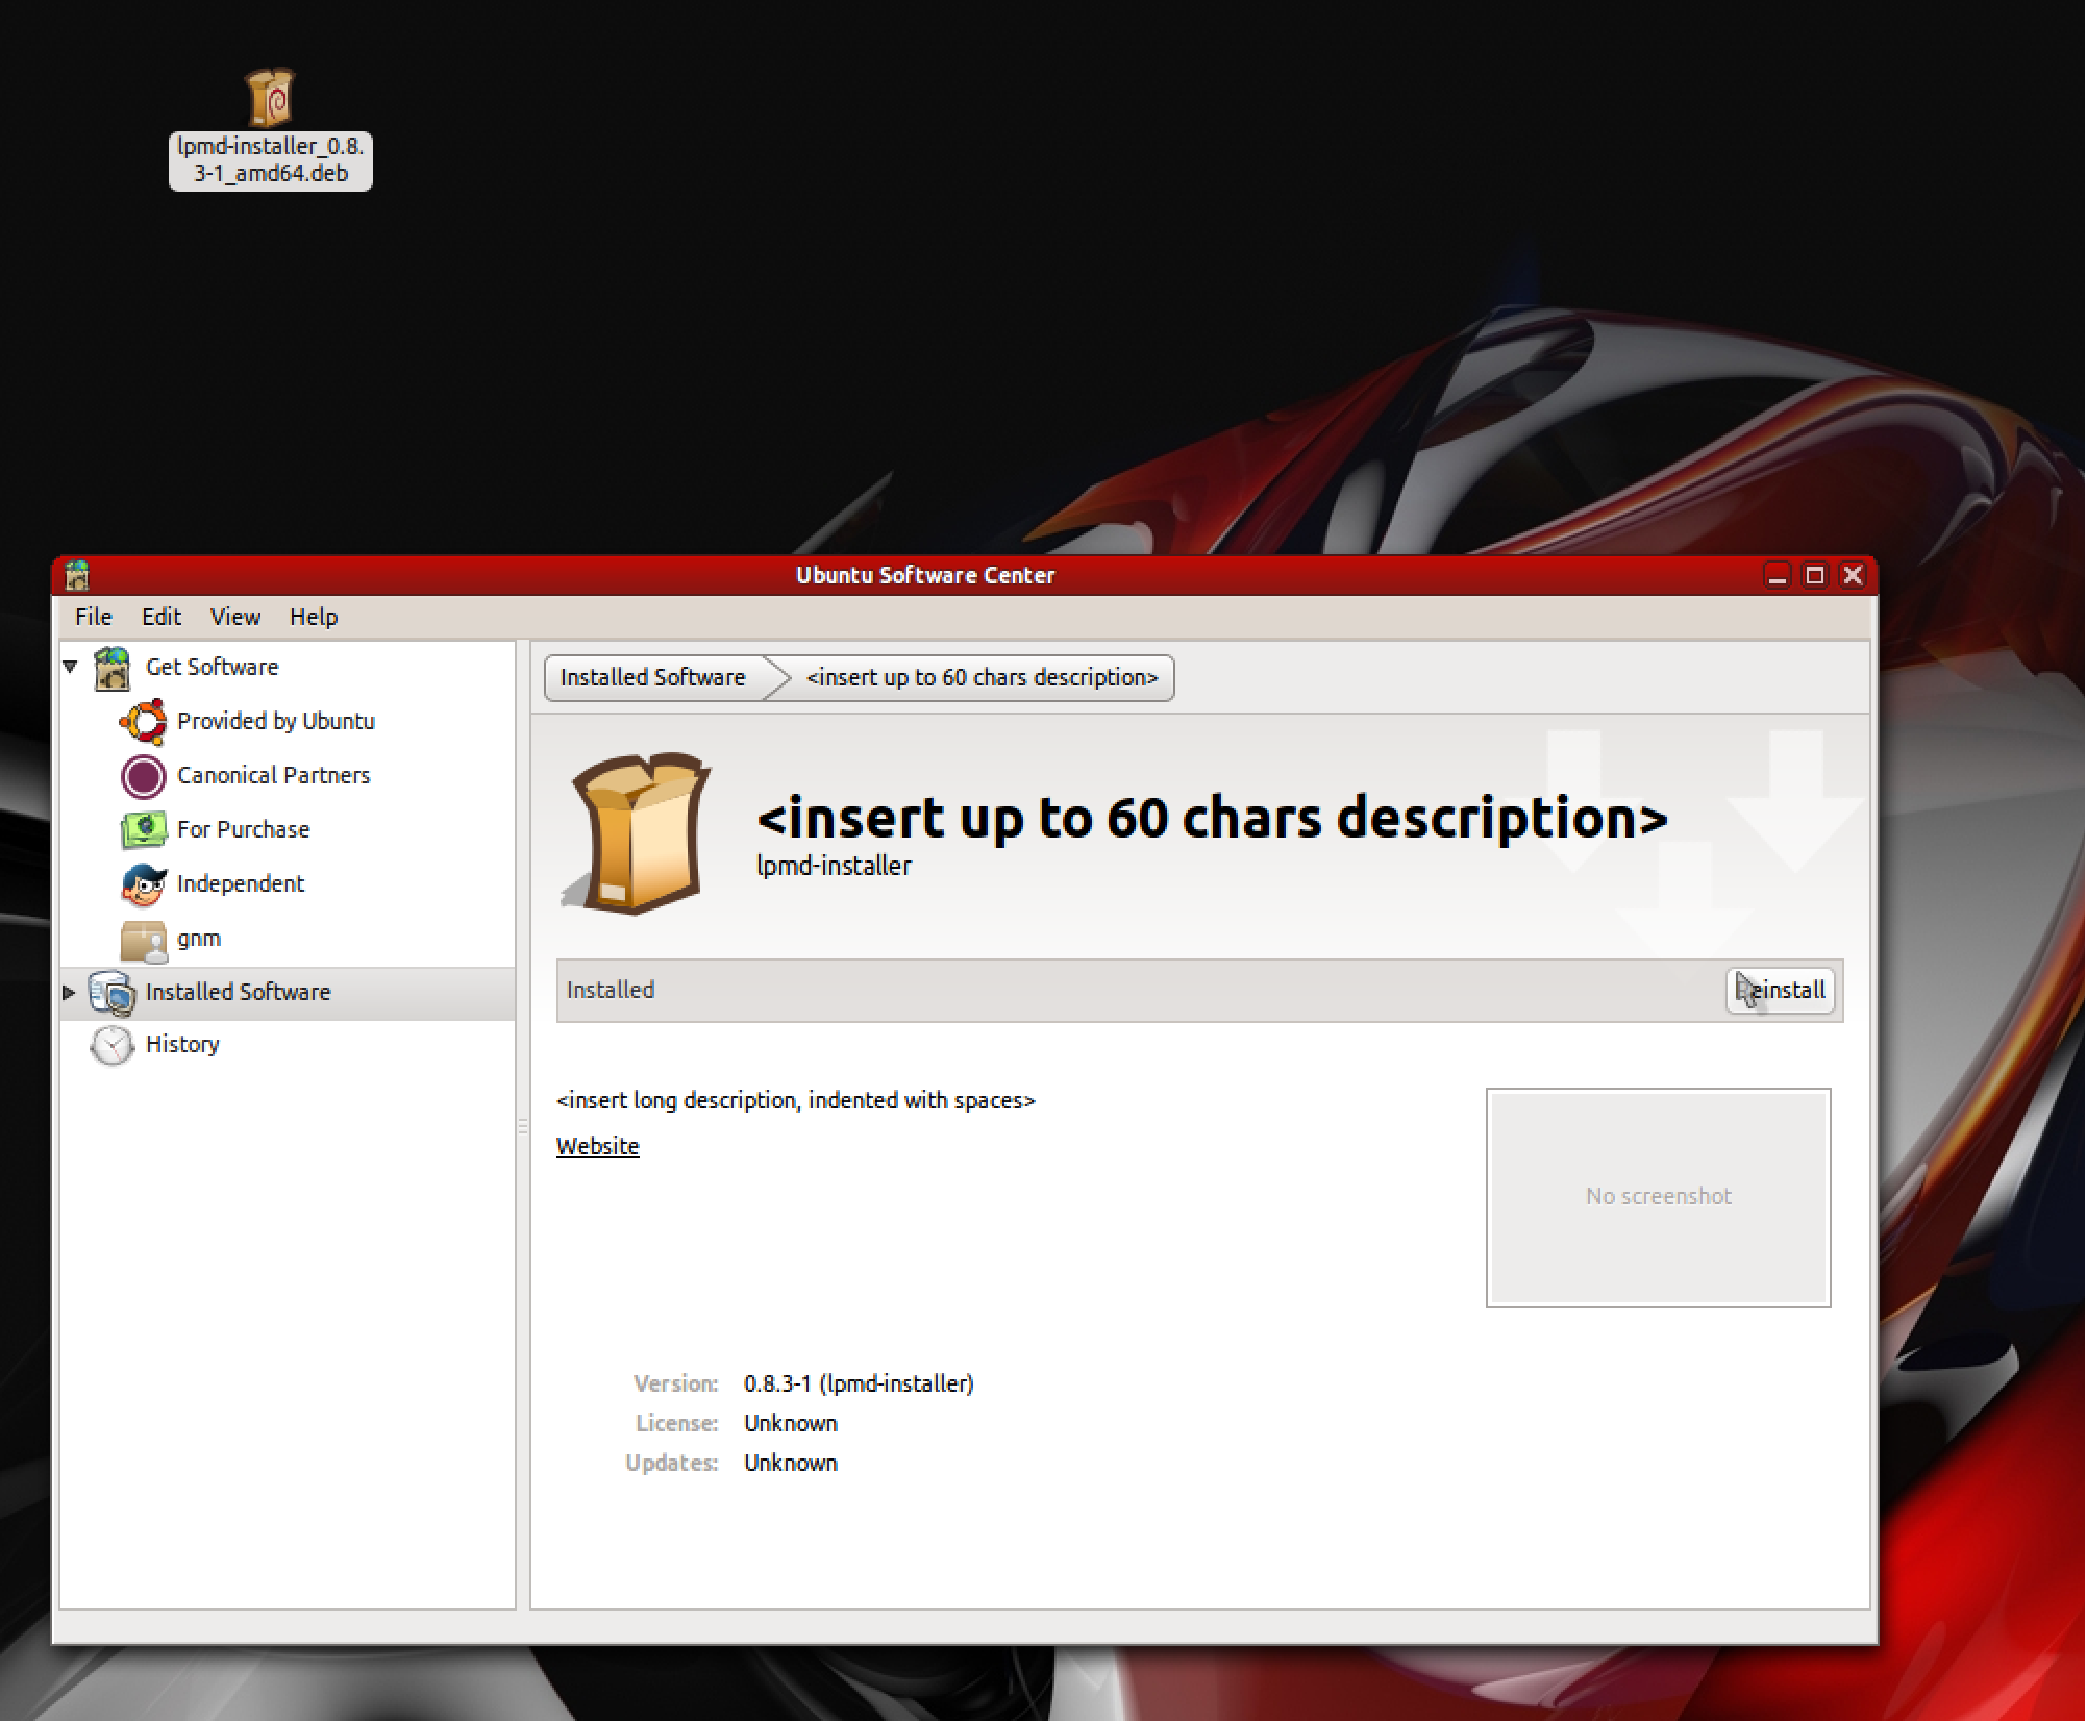
\includegraphics[scale=.20]{installer-package-2.pdf}
 \label{fig:installer-package-2}
}
\caption{If you make double click to the package the installation process of
the lpmd-installer package will begin.}
\label{fig:lpmd-installer}
\end{figure}

\subsubsection{Debian based distributions - adding repository}
At first place, as administrator, edit the file \verb|\etc\apt\sources.list|
and add the following lines.

\begin{verbatim}
 #GNM Repositories
 deb http://arpa.ciencias.uchile.cl/repo/ gorilla main
\end{verbatim}

You can make the same procedure in a Ubuntu distribution using directly the
software center and adding the software source adding :

\begin{itemize}
 \item Type : Binary
 \item URL : http://arpa.ciencias.uchile.cl/repo/
 \item Distribution : gorilla
 \item Components : main
 \item Comment : A GNM source/binary distribution.
\end{itemize}

\begin{figure}[h!]
\centering
 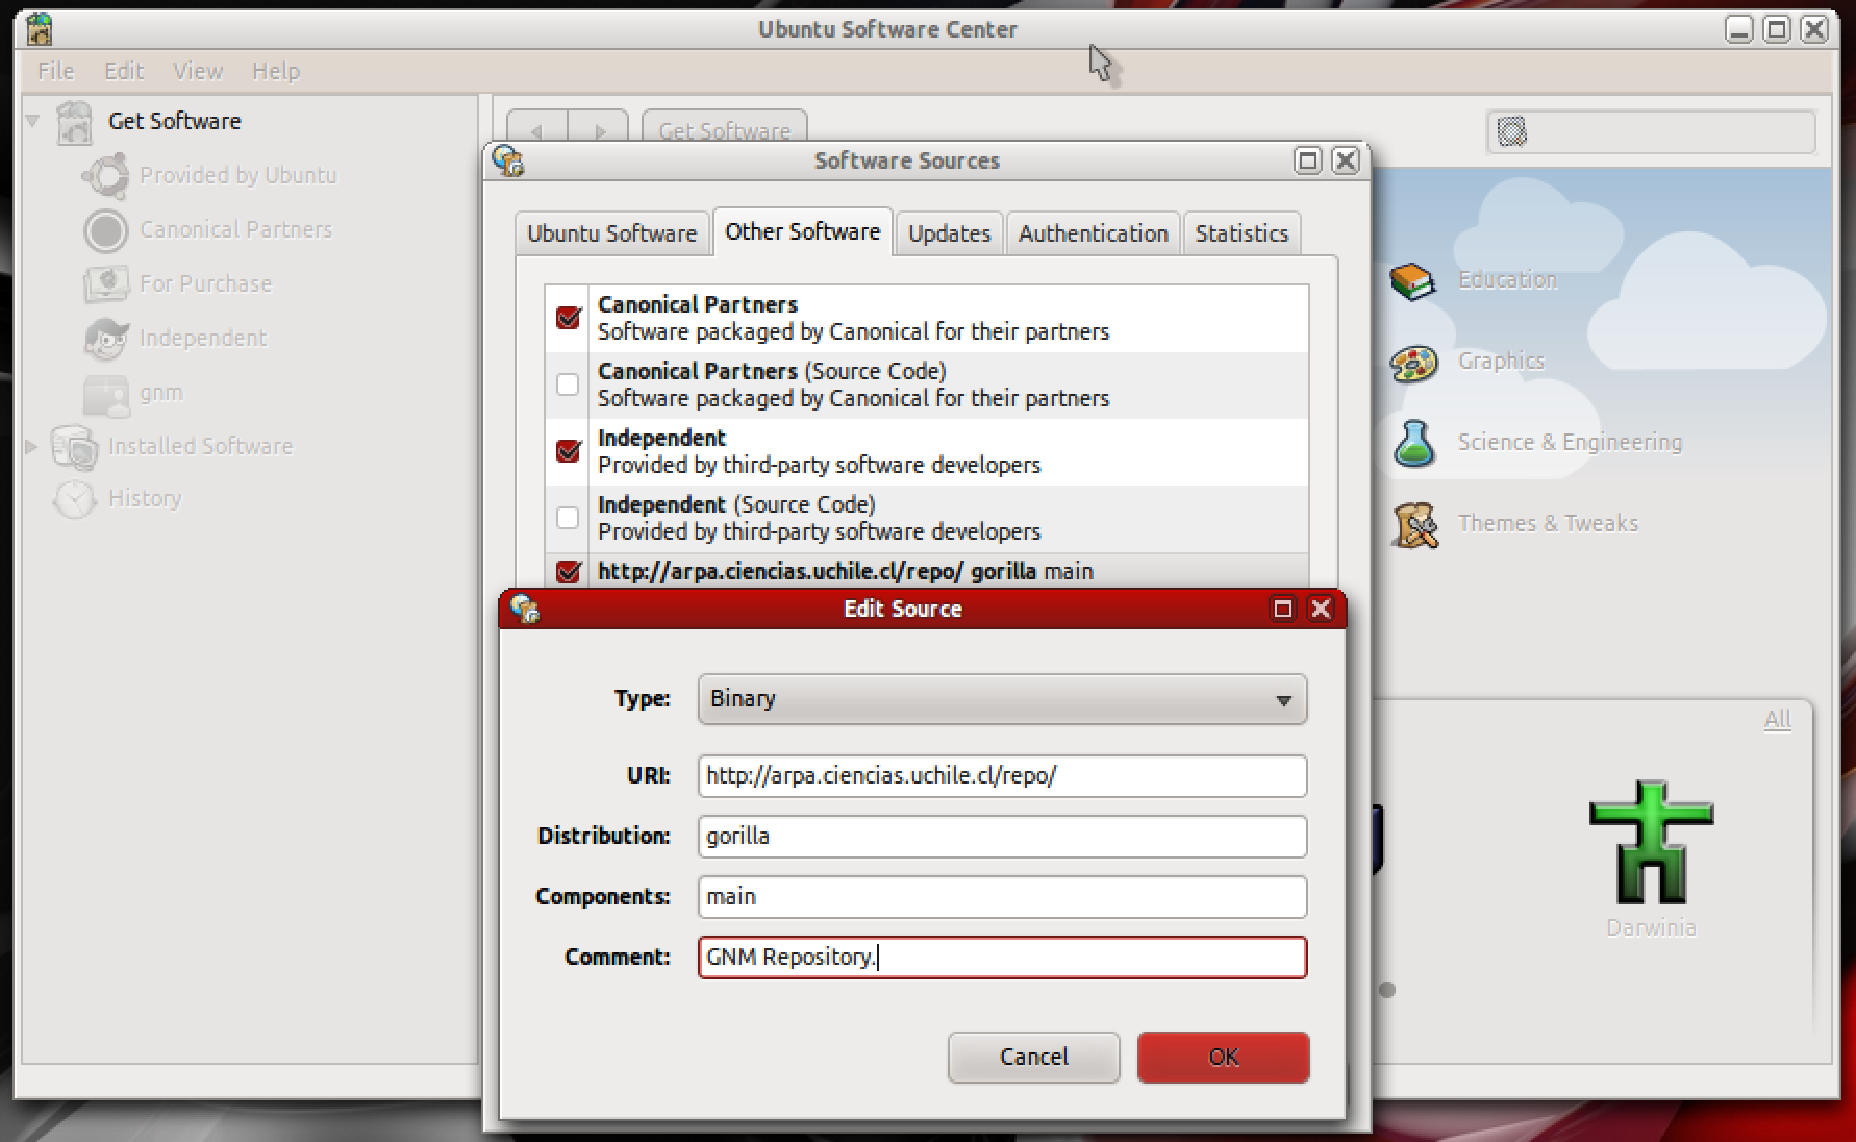
\includegraphics[scale=.35]{repository.pdf}
\caption{Setting the repositories in a ubuntu distribution.}
\label{fig:repository}
\end{figure}

\noindent
the figure~\ref{fig:repository} show how to setup the repository in a ubuntu
distribution in order to install the \verb|lpmd-installer| package.

Finally, as administrator execute :
\control{
 apt-get update\\
 apt-get install lpmd-installer
}

Now check that you have the \verb|lpmd-installer| command :
\begin{verbatim}
 username@machine:~$ lpmd-installer 
 lpmd-installer [ -i <branch or version> | -u ] [-v] [-p <prefix>] [-P <package>] 
                [-s <server>] [-S <suffix>] [ -d <sources dir>] [-t]
 username@machine:~$
\end{verbatim}

Great! you are ready to install {\lpmd} easily.

\subsubsection{Others Distributions}

In order to install \verb|lpmd-installer| in distributions non based on Debian,
is necessary download the program directly from internet, you can found the
program here :\\

\url{http://www.gnm.cl/lpmd/uploads/Main/lpmd-installer}\\

Download the file and change the execution permission of the file :

\begin{verbatim}
 chmod 755 lpmd-installer
\end{verbatim}

Afther that, you can copy or move the file to some plece where you have set the
\verb|PATH| environment variable. In mostly of the system *nix is enoguh copy to
:

\begin{verbatim}
 cp lpmd-installer /usr/local/bin/
\end{verbatim}

And this is it, now check that you have the \verb|lpmd-installer| command
available in your system.
\begin{verbatim}
 username@machine:~$ lpmd-installer 
 lpmd-installer [ -i <branch or version> | -u ] [-v] [-p <prefix>] [-P <package>] 
                [-s <server>] [-S <suffix>] [ -d <sources dir>] [-t]
 username@machine:~$
\end{verbatim}

Great! you are ready to install {\lpmd} easily.

\subsection{Testing lpmd-installer}

\verb|lpmd-installer| have all necessary in order to install {\lpmd} in a
system or in personal accounts, like as facilities fo install external
\textit{plugins}, like \verb|lpvisual|. Between the principal options of
\verb|lpmd-installer| we have :

\begin{itemize}
 \item \verb|-l| : Show all version available to install.
 \item \verb|-p| : Espcify the path to install lpmd(prefix).
 \item \verb|-P| : What package you will install.
 \item \verb|-d| : Set where the sources will be, if you don't set this values
the sources are deleted after the installation process.
 \item \verb|-u| : Update the {\lpmd} version that you have in your system.
\end{itemize}

Below, we will show you how to install {\lpmd} using \verb|lpmd-installer|.

\subsection{Installing lpmd on the system using lpmd-installer}

Before run the installation process of {\lpmd} in the system, we recommend that
you take a look of the available versions in the principal server, for this
just run \verb|lpmd-installer -l|, and you will se a list with the packages,
like this :

\begin{verbatim}
username@machine:~$ lpmd-installer -l
These are the available versions of package lpmd:

From branch 0.5: 
    0.5.4-delta2
    0.5.4

From branch 0.6: 
    0.6.1

From branch testing: 
    svn
username@machine:~$
\end{verbatim}

You have to choose wath version do you want install, in this case we will
consider the version 0.6.1, if we try to install in the system without
administrator permissions, you will have a message like this :

\begin{verbatim}
username@machine:~$ lpmd-installer -i 0.6.1
Preparing to install lpmd 0.6.1
[Error] You do not have permission to install on /usr/local
username@machine:~$
\end{verbatim}

This happen because, {\lpmd} by default try to be installed in
\verb|/usr/local| and a normal user have not privileges to write in this
folder. The right way to proceed is, install as a administrator. For this :

\begin{verbatim}
username@machine:~$ sudo -s
[sudo] password for username: 
root@machine:~# lpmd-installer -i 0.6.1
\end{verbatim}

Now, the process will begin in automatic way to download from the principal
server the necessary packages to install {\lpmd}. Remember that you will
request at least one \verb|C++| compiler in order to realize the installation.
By the other hand we suggest that you have too installed the \verb|zlib|
library, in mostly of the *nix system is called \verb|zlib1g-dev|, for to this
in Debian based dsitribution, the preocedure will be :

\begin{verbatim}
username@machine:~$ sudo -s
[sudo] password for username: 
root@machine:~# apt-get install zlib1g-dev
\end{verbatim}


\subsection{Installing lpvisual with lpmd-installer}

With \verb|lpmd-installer| you can realize the installation of the
\verb|lpvisual| plugin, this is a independient plugin based in OpenGL and is
used for the visualization of atomic configurations of different types. For a
right compilation of the source code, you will need install the principal
libraries of the OpenGL project, for this, in Debian based distribution you can
use :

\begin{verbatim}
username@machine:~$ sudo -s
[sudo] password for username: 
root@machine:~# apt-get install libglut3-dev
\end{verbatim}

Now, to install \verb|lpvisual| at the system you can use the same options of
\verb|lpmd-installer| used previously :

\begin{verbatim}
username@machine:~$ lpmd-installer -P lpvisual -l
These are the available versions of package lpvisual:

From branch 2.0: 
    2.0svn
username@machine:~$  
\end{verbatim}

So, we will choose the version of \verb|lpvisual| that you want install, and
you install this easly with :

\begin{verbatim}
username@machine:~$ lpmd-installer -P lpvisual -i 6.0
....
\end{verbatim}

With this you installed an additional plugin using the lpmd-installer package.

\subsection{Installing lpmd in a personal account}

Sometimes, the user is not an system administrator, under this, you can install
{\lpmd} in a persinal account, for that \verb|lpmd-installer| have additional
flags that you can use for this. Take in acount an example, supouse that you
want install {\lpmd} in a local folder, for example \verb|~/local|. For this
installation process is necessary day where is the directory using the flag
\verb|-p| as :

\begin{verbatim}
username@machine:~$ lpmd-installer -i 0.6.1 -p /home/username/local
....
username@machine:~$
\end{verbatim}

With this command we installed {\lpmd} en the personal account, we can also
choose the possibility to keep the source code in other directory, for example
using :

\begin{verbatim}
username@machine:~$ lpmd-installer -i 0.6.1 -p /home/username/local -d /home/username/sources
....
username@machine:~$
\end{verbatim}

For user support and more tips about \verb|lpmd-installer| yo can send an
e-mail to the developers or visit the web-page of the project in
\url{http://www.lpmd.cl}.

\section{Download without lpmd-installer}
\label{sec:descarga}

If you choose do not install {\lpmd} using the \verb|lpmd-installer| program,
then you have to download the three principal packages in order to install
{\lpmd}. You can choose two different version, the last stable version or the
developer version, in both you will have to download all the three packaes, the
\verb|API|, the plugins set and the executables (with utilities).

%%%%%%%%%%%%%%%%%%%%%%%%%%%%%%%%%%%%%%%%%%%%%%%%%%%%%%%%%%%%%%%%%
%%%%%%%%%%%%%%%%%%%%%%%%%%%%%%%%%%%%%%%%%%%%%%%%%%%%%%%%%%%%%%%%%
\subsection{Download the last stable version}

The last stable version of {\lpmd} packages are :

\begin{itemize}
 \item liblpmd : ver. 0.2.2
 \item plugins : ver. 0.2.2
 \item lpmd    : ver. 0.6.2
\end{itemize}

You can download this in the web page \url{http://www.lpmd.cl} or request them 
by e-mail. The webpage \textbf{always} is more updated that this document.

%%%%%%%%%%%%%%%%%%%%%%%%%%%%%%%%%%%%%%%%%%%%%%%%%%%%%%%%%%%%%%%%%
%%%%%%%%%%%%%%%%%%%%%%%%%%%%%%%%%%%%%%%%%%%%%%%%%%%%%%%%%%%%%%%%%
\subsection{Download the last updated development version}

For the people that are interested in use tha last version, including last
updates, mprovements and bug correction, can download the last updated
development (LUD) version in the web-page.

\url{http://www.lpmd.cl/testing}

The installation procedure for this packages is similar to the last stable
version that is showed in section~\ref{sec:withoutinstaller}.

\section{Installation without lpmd-installer}
\label{sec:withoutinstaller}

In order to install {\lpmd} without using \verb|lpmd-installer| the first step
is install the \verb|API| of the project before install any other package. The
order for the next installation packages will be no important.

% \fb{
% \begin{minipage}[l]{10cm}
% Nota : Los que poseen la versi\'on testing/unstable cuentan con \texttt{NMC}
% (\textit{NanoMaterialsConfigure}) una utilidad desarrollada por Sergio Davis
% en % python, similar al ya conocido \texttt{configure} de GNU pero mucho m\'as
% ajustado a nuestros requerimientos.
% \end{minipage}
% }

%%%%%%%%%%%%%%%%%%%%%%%%%%%%%%%%%%%%%%%%%%%%%%%%%%%%%%%%%%%%%%%%%
%%%%%%%%%%%%%%%%%%%%%%%%%%%%%%%%%%%%%%%%%%%%%%%%%%%%%%%%%%%%%%%%%
\subsection{Installing the liblpmd API}

At first, uncompress the package of \textbf{liblpmd}.

\control{tar -xvzf liblpmd-X.X.X.tar.gz}

This will generate a new folder. In order to install this library with all the
necessary issues for the good operation of {\lpmd}, execute :

\control{./setup \\ make}

and with administrator privileges,

\control{make install}

By \textit{default} the installation folder of the \verb|API| is
\verb|/usr/local|, in the case that you need locate the api in a different
folder, set this using the \verb|--prefix| option in the \verb|./setup|
process. And in particular if you want install {\lpmd} in your personal home
check the section~\ref{subsub:personaldir}.

In case of error messages or any other problems during the installation of the
\verb|API| package, please send an e-mail to the developers or to
\verb|gnm@gnm.cl|.

%%%%%%%%%%%%%%%%%%%%%%%%%%%%%%%%%%%%%%%%%%%%%%%%%%%%%%%%%%%%%%%%%
%%%%%%%%%%%%%%%%%%%%%%%%%%%%%%%%%%%%%%%%%%%%%%%%%%%%%%%%%%%%%%%%%
\subsection{Installing plugins}

One of the basic requeriments in the installation process of {\lpmd} is have a
well defined location of the plugins that {\lpmd} will use. If the \verb|API|
package was installed in a standard way, you can configure and install plugins
easily using :

\control{./setup  \\ make}

and with administrator privileges, run :

\control{make install}

With this standard procedure, all the plugins will be installed in the folder
\verb|/usr/local/bin/lpmd|. If you install the \verb|API| in a different
location using the \verb|--prefix| option, we suggest that you use the same
place for the plugin using the same option in the \verb|./setup| command.

%%%%%%%%%%%%%%%%%%%%%%%%%%%%%%%%%%%%%%%%%%%%%%%%%%%%%%%%%%%%%%%%%
%%%%%%%%%%%%%%%%%%%%%%%%%%%%%%%%%%%%%%%%%%%%%%%%%%%%%%%%%%%%%%%%%
\subsection{Installing lpmd}

This is the smaller and faster packages to install. Is similar to the previous
packages, if you use the standard procedure and location, execute :

\control{./setup \\ make}

and with administrator privileges, run :

\control{make install}

If you choose a different location for the \verb|API|, we suggest that use this
location too in the \verb|./setup| process for the final package, for this you
can use the \verb|--prefix| option too.

Finally you will have a set of different executables availables, \verb|lpmd|,
\verb|lpmd-analyzer|, \verb|lpmd-converter|, \verb|lpmd-visualizer| and
\verb|lpmd-plotter| availables in your system. In a standard installation
process this executables are installed in \verb|/usr/local/bin/|, if you
install {\lpmd} in a different folder please correct your \verb|PATH| in order
to have acces to the executables.

You can run {\lpmd} using :

\begin{verbatim}
username@machine:~$ lpmd
...
LPMD version 0.6.1
Using liblpmd version 2.0.1

Usage: lpmd [--verbose | -v ] [--lengths | -L <a,b,c>] [--angles | 
-A <alpha,beta,gamma>] [--vector | -V <ax,ay,az,bx,by,bz,cx,cy,cz>] 
[--scale | -S <value>] [--option | -O <option=value,option=value,...>] 
[--input | -i plugin:opt1,opt2,...] [--output | -o plugin:opt1,opt2,...] 
[--use | -u plugin:opt1,opt2,...] [--replace-cell | -r] [file.control]
       lpmd [--pluginhelp | -p <pluginname>]
       lpmd [--help | -h]
\end{verbatim}

% \subsection{Typical post-installation problems}
% 
% In this section you will found the more typical post-installation error
% related
% to {\lpmd} installation process.
% 
% \subsubsection{Loading library error}
% 
% This is the more typical installation process in the 0.5 branch of {\lpmd}.
% After the installation process of {\lpmd} you will se only a Error of a error
% refering to liblpmd library can't be found.
% 
% The fast way to correct this problem is,
% 
% \begin{itemize}
%  \item Edit /etc/ld.so.conf
%  \item Add the line /usr/local/lib to the file.
%  \item Run with administrator privileges: ldconfig
% \end{itemize}
% 
% Now you will can run \verb|lpmd| without problems, if you still having
% problems, please report these to the developers.

% \subsection{Instalaci\'on de lpmd en directorio personal}
% \label{subsub:personaldir}
% 
% Podemos instalar cada uno de los paquetes (\textbf{liblpmd}, \textbf{plugins}
% y \textbf{lpmd}) en un directorio personal, para eso consideremos un ejemplo,
% en % el cual deseamos instalar estos paquetes en el directorio \verb|local|
% ubicado % en el \textit{home} del usuario, el procedimiento ser\'ia:
% 
% \begin{itemize}
%  \item Para liblpmd :
%  \begin{verbatim}
%  ./setup --prefix=/home/user/local
%  make
%  make install
%  \end{verbatim}
%  \item Para plugins :
%  \begin{verbatim}
%  ./setup --prefix=/home/user/local
%  make
%  make install
%  \end{verbatim}
%  \item Para lpmd :
%  \begin{verbatim}
%  ./setup --prefix=/home/user/local
%  make
%  make install
%  \end{verbatim}
% \end{itemize}
% 
% De esta forma se generar\'an los esqueletos en \verb|/home/user/local| con
% \verb|bin|, \verb|lib|, etc. Ahora puede ejecutarlos si su \verb|PATH| esta
% bien % configurado a la direcci\'on \verb|/home/user/local/bin|.


%%%%%%%%%%%%%%%%%%%%%%%%%%%%%%%%%%%%%%%%%%%%%%%%%%%%%%%%%%%%%%%%%
%%%%%%%%%%%%%%%%%%%%%%%%%%%%%%%%%%%%%%%%%%%%%%%%%%%%%%%%%%%%%%%%%
\subsection{Update the lpmd packages}

In order to update your actual version of {\lpmd} in your system. You have two
alternatives. The first one is using the normal installation process explained
in the section~\ref{sec:withoutinstaller} and overwrite your actual version.

The second procedure in order to update your actual version of {\lpmd} is using
the \verb|lpmd-installer| package. The procedure to update your installation is
easy, only type:

\begin{verbatim}
 lpmd-installer -u
\end{verbatim}
\noindent
With this an automatic process will be start using the last update version of
{\lpmd}.
